% !TeX spellcheck = en_EN-English

\section{Embedding of Patient}
\label{embeddingImple}

First of sub-tasks for prediction of patient future costs is to embed each patient record into numerical vector that would be understandable for neural network. For each record of a patient we embed four information. First and easy to implement is a timestamp which is computed using numerical and date values, then there three more tricky information and those are diagnosis, medical procedure and prescribed drug. 

\subsection{Timestamp}
\label{timespampImple}

To compute timestamp we first took all records for single patient and found one with earliest date. This record is then used as pivot for computation of all timestamp for patient. To compute timestamp for this record we took age of patient in years add half year and multiplied it by 365 to get approximate age of patient in days which served as a timestamp, we add half a year in order to improve approximation since we have only age in years meaning we don't know whether they had birthday one or eleven months ago, however we expect it to be on average six months so half of a year. For all subsequent records we compute difference between date of record and date of first record in days and add this difference to timestamp from first record to create one for this record. 

\subsection{Diagnosis embedding}

As discussed in Sec. \ref{diagEmb} embedding of diagnose is based on MKCH-10-SK (ICD-10-CM) code of disease. Where we split this code into three parts and embed each other independently and finally concatenate result.
\\

To embed main category we generated vector containing random numbers using uniform distribution for each letter of English alphabet we choose to sample these random numbers from interval [-0.5, 0.5]. We choose this interval mostly arbitrarily since we were planing to pass recording embedding into normalization function once it complete.
\\

For subcategory and details we linearly assigned value to each possible two digit code. We chose interval from which we take this value to be [-0.5, 0.5], meaning subcategory 00 would get -0.5 category 50 would get 0 and category 99 would get 0.5, this interval was chosen in order to for each dimension of this embedding to have same mean and standard deviation as each dimension of main category. Thanks to that they also have on average same distance per dimension. This means that each position of each part of embedding should contribute to total distance with same weight.
\\

Most important part was to assign lengths to vector of each part in a way that would encode their importance. 
Main category, the most important part, got vector of length 28, subcategory part got length 7 and finally details got length 3.
\\

Showcase of resulting embedding can be seen on Fig. \ref{fig:diag_emb_show} where each part is highlighted by different color and all values are rounded to two decimal.

\begin{figure}[!h]
	\centering
	
	% TODO image needs update after change of lengths of each embeddings
	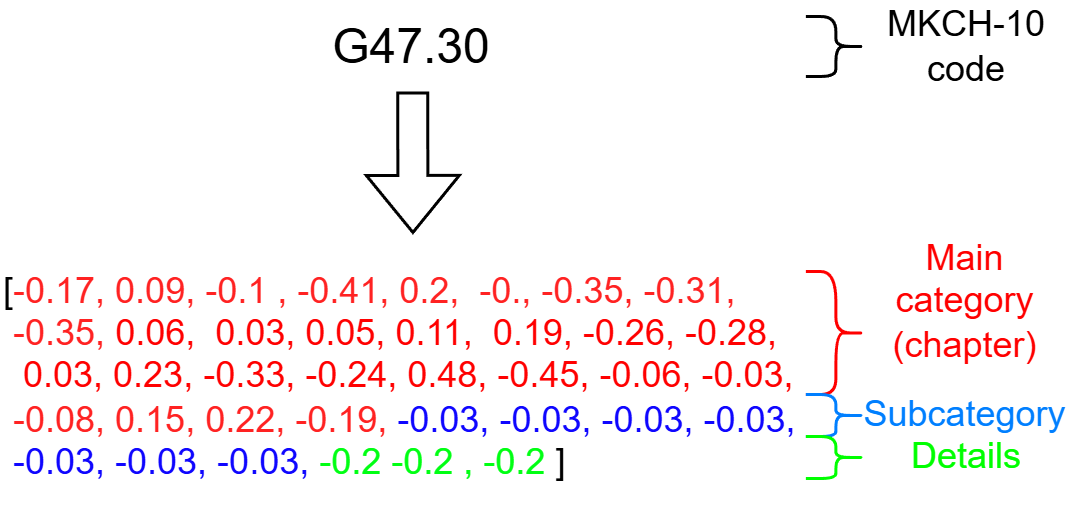
\includegraphics[width=0.8\textwidth]{images/diagnosis_embed_showcase.png} 
	
	\caption{Showcase of resulting embedding of specific diagnosis (rounded to two decimal places).}
	\label{fig:diag_emb_show}
\end{figure} 


\subsection{Drug embedding}

Embedding was done in very similar way as in diagnosis embedding, meaning each level was embedded separately and final embedding was done as concatenations of them. In this case each level was embed using random vector from uniform distribution with interval [-0.5, 0.5]. We used random vectors for each level since none of levels contains any internal sub-groupings similar to subgroups of diagnosis (see Sec. \ref{mkch_subdiv} subgroup codes). To encode importance of levels we again used lengths of random vectors, where with higher level vectors shortens. Lengths of vectors for each level can be seen in Tab. \ref{tab:drug_lev_len}. So total length of embedding is same as embedding for diagnosis.In case code is incomplete, meaning it's missing higher levels, missing part is substituted with zeros which we consider neutral elements.
\\

\begin{table}[!h]
	\centering
	\begin{tabular}{|l|l|}
		\hline
		Level  & Length \\ \hline
		1 & 21 \\ \hline
		2 & 9 \\ \hline
		3 & 5 \\ \hline
		4 & 2 \\ \hline
		5 & 1 \\ \hline
	\end{tabular}
	\caption{Lengths of random vectors assigned to each information level of ATC code.}
	\label{tab:drug_lev_len}
\end{table}  

With this embedding we should get codes whose similarity is more dependent on whether lower more important levels match than higher ones.

\subsection{Medical procedure embedding}

Embedding of medical procedure was straightforward since we used already trained model. 
\\
%In case of LLM model we inputted complete medical procedure descriptions into model to generate their embeddings, and then took those embedding and performed principal component analysis (PCA) on them to decrease dimensionality while retaining most of variance, in other words information, from original embedding. In case of Word2vec model we firstly
%\\

As discussed in \ref{procedureEmb}, for LLM we choose LaBSE model. It's a model developed by Goggle to encode text into high dimensional vectors. This model was trained 109 languages including Slovak.  Using this model was straightforward and we just had to input complete description of procedure into to receive 768 dimensional dense encoding of it. After computing all embedding we performed principal component analysis (PCA) to reduce dimensionality of this embedding while maintaining most of the variance or in other words most of the information stored inside it.
\\

We tried also different approach using Word2vec model trained specifically for Slovak language. More specifically we used word2vec-sk model made by company Essential Data \cite{w2v}. This model was trained on corpus containing around 110 millions of words. More specifically we choose version of model trained using CBOW approach. Since this model is trained to embed words not a text, we firstly split description of procedure into words and lemmatize those words, in other word change into their base form, then using Word2vec model we embed each word into dense 200 dimensional vector separately and finally create description embedding as an average of embeddings of all words in it.
\\

We expected that LaBSE model produce better results compared to standard text embedding models trained solely on Slovak language, since LaBSE model is during training comparing embedding not only to similar sentences in Slovak language but also their translation in other which could mitigate a relatively small amount of Slovak language data compared to other more commonly used languages. Additionally this model could know domain specific words in our case medical terms which are left in foreign language and would most likely not be found in Slovak only corpus. 
\\

Finally we create record embedding by concatenating all four parts. Since we have two separate datasets, one for prescribed drugs and one for medical procedures, we always have only three out of four information available for each record, since timestamp and diagnosis are always available, we substitute missing part with vector of zeros with appropriate length which is most neutral embedding since we centered both medical procedure and drug prescription embedding around zero.
